\documentclass{beamer}
\usetheme{afm}

\title{Interest Rate Derivatives}
\subtitle{Main IR Contracts Theory}
\course{Advanced Financial Modeling}
\author{\href{mailto:matteo.sani@unisi.it}{Matteo Sani}}

\begin{document}
	\begin{frame}[plain]
		\maketitle
	\end{frame}
	
\section{Forward Rate Agreement}
\begin{frame}{Forward Rate Agreement}{Definition}
	\begin{itemize}	
		\item<1-> A \textcolor{red}{Forward Rate Agreement} (FRA) is a contract involving three time instants: %the current time $t$, the fixing time $T>t$, and the maturity time $S>T$.
		\begin{equation*}
			\underbrace{t}_{\text{current time}} \leq \underbrace{T}_{\text{fixing time}} \leq\underbrace{S}_{\text{maturity}}
		\end{equation*}
		\item<2-> The FRA payout consists of an exchange of interest rate flows calculated for the time period $\tau=S-T$. At the maturity $S$, a fixed payment based on a fixed rate $K$ is exchanged against a floating payment based on the spot rate $L(T, S)$ whose value is known only in $T$.
		\item<3-> Basically, this contract allows one to lock-in the interest rate between times $T$ and $S$ at a desired value $K$. (\textbf{Note:} interest rate flows are calculated using the simple compounding law).
	\end{itemize}
\end{frame}

\begin{frame}{Forward Rate Agreement}
	\begin{itemize}
	\item<1-> A FRA is an agreement that enables a user to \emph{hedge} itself against unfavorable movements in interest rates by fixing a rate on a notional amount that is (usually) of the same size and term as its exposure that starts sometime in the future. 
	\item<2-> Consider a $3\times 6$ FRA (3-month into 6-month): the 3 in the $3\times 6$ refers to 3 months' time when settlement (fixing) takes place, and the 6 to the expiry date of the FRA from deal date, i.e. the rate quoted for the FRA is a 3-month rate at the time of settlement
	\end{itemize}
\end{frame}

\begin{frame}{FRA Example}
	\begin{center}
		\includegraphics[width=0.9\linewidth]{FRA_diagram}
	\end{center}
\end{frame}

\begin{frame}{FRA: Formalization of the Contract}
	\begin{itemize}
		\item<1-> Formally, at time $S$ one receives $\tau(T, S)KN$ units of currency and pays the amount $\tau(T,S)L(T,S)N$, where $N$ is the contract nominal value.
		\item<2-> Thus, at time $S$, the future (and today unknown) payout of the contract is: 
		\begin{equation}
			N\tau(T,S)(K-L(T,S))
			\label{eq:fra_payoff}
		\end{equation}
		\item<3-> In order to assign a value at this contract we have to tackle two issues:
		\begin{itemize}
			\item<4-> estimate the future value of $L(T, S)$;
			\item<5-> discount the result from $S$ to today (time $t$).
		\end{itemize}
		\item<6-> There are several ways to arrive at the final result: \textbf{no arbitrage is the common denominator.}
	\end{itemize}
\end{frame}

%\begin{frame}{FRA: Numerical Example}
%	A company enters into a FRA to receive 4\% on \$100M for a 3-month period starting in 3 years. Imagine that LIBOR is 4.5\% in 3 years.
%	
%	So $T=3y$, $S=3.25y$, $K=4\%$, and $L(T,S)=4.5\%$.
%	
%	The net cash-flow at time $S$ is
%	\begin{equation*}
	%		100000000\times(0.04-0.045)\times0.25 = -\$125000
	%	\end{equation*} 
%\end{frame}

\subsection{FRA Valuation}
\begin{frame}{FRA: the Standard Derivation}
	\begin{itemize}
		\item<1-> Following the approach reported in Brigo-Mercurio (2006) we can proceed as follows.		
		\only<2-2>{
		\item Substitute in \cref{eq:fra_payoff} $L(T,S)$ with its expression as a function of the zero-coupon bond price $P$ and get
		\begin{equation*}
			N\bigg[\tau K + 1 - \frac{1}{P(T, S)}\bigg]
		\end{equation*}
		}
		\only<3-3>{
		\item Substitute in \cref{eq:fra_payoff} $L(T,S)$ with its expression as a function of the zero-coupon bond price $P$ and get
		\begin{equation*}
			N\bigg[\tau K + 1 - \underbrace{\frac{1}{P(T, S)}}_{A}\bigg]
		\end{equation*}
		}
		\item<3-> First interpret $A$ as an amount of money held at time $S$. At $T$ it's worth 1, indeed 
		\begin{equation*}
			A = P(S,S)A \implies P(T,S)A = P(T,S)\frac{1}{P(T,S)}=1
		\end{equation*}
		which in turn, at time $t$, equals to
		\begin{equation*}
			P(t,T) 1 = P(t,T)
		\end{equation*}
	\end{itemize}
\end{frame}

\subsection{FRA Valuation}
\begin{frame}{FRA: the Standard Derivation}
	\begin{itemize}
		\item<1-> Following the approach reported in Brigo-Mercurio (2006) we can proceed as follows.		
		\item Substitute in \cref{eq:fra_payoff} $L(T,S)$ with its expression as a function of the zero-coupon bond price $P$ and get
		\begin{equation*}
			N\bigg[\underbrace{\tau K + 1}_{B} - \underbrace{\frac{1}{P(T, S)}}_{A}\bigg]
		\end{equation*}
		\item<1-> On the other hand $B$ in $S$ becomes at time $t$:
		$P(t,S)\tau K + P(t, S)$.
		\item<3-> Collecting the terms we get
		\begin{equation}
			\textbf{FRA}(t,T,S,\tau,N,K)=N[P(t,S)\tau K–P(t,T)+P(t,S)]
		\end{equation}
	\end{itemize}
\end{frame}

\subsection{FRA Valuation ($2^{nd}$ Approach)}
\begin{frame}{FRA Valuation: a Different Approach}
	Now we will try to estimate the value of a FRA using a simple replication approach:
	\begin{itemize}
		\item<1-> at time $t$: 
		\begin{equation*}
			\begin{cases}
				\text{lend}~P(t,T)\\
				\text{borrow}~P(t,S)(1+\tau(T,S)K)
			\end{cases};
		\end{equation*}
		\item<3-> at time $T$: you receive 1 which you will invest at the (in $t$ unknown) EURIBOR rate $L(T,S)$;
		\item<4-> at time $S$: 
		\begin{equation*}
			\begin{cases}
				\text{receive}~(1+L(T,S)\tau(T,S))\\
				\text{pay}~1 + \tau(T,S)K
			\end{cases}.
		\end{equation*}
	\end{itemize}
\end{frame}

\begin{frame}{FRA Valuation: a Different Approach}
	Adding the cash-flows together and evaluating in $t$ we get:
	\begin{equation*}
		1+L(T,S)\tau - 1 - \tau K = (L(T,S)-K)\tau
	\end{equation*}
	\uncover<2->{From the risk-neutral pricing formula
	\begin{equation*}
	\mathbb{E}^Q[D(t, S)(L(T, S)-K)\tau(T,S)|\mathcal{F}_t]
	\end{equation*}
	}
	\uncover<3->{According to the \emph{Fundamental Theorem II} its value must equal to the value of the replicating portfolio in $t$ (we assume to be in a complete market). Hence
	\begin{equation}
		\begin{aligned}
			\mathbb{E}^Q[D(t,S)&(L(T,S)-K)\tau(T,S)|\mathcal{F}_t]=\\
			&[P(t,S)\tau(T,S)K-P(t,T)+P(t,S)]
			\label{eq:fra_as_expectation}
		\end{aligned}
	\end{equation}
    }
\end{frame}

\subsection{FRA Detailed Proof}
\begin{frame}{FRA Detailed Proof I}
\begin{itemize}
	\item<1-> Let's start from the risk neutral pricing formula
	\begin{equation*} \textbf{FRA} = 
\mathbb{E}^\mathcal{Q}_t[D(t,S)\tau (K - L(T,S))] = 	\mathbb{E}^\mathcal{Q}_t[D(t,S)\tau K - D(t,S)\tau L(T,S)]
	\end{equation*}
	\item<2-> From which we can easily derive
	\begin{equation*}
		\begin{aligned}
		\textbf{FRA} = \tau &K\mathbb{E}_t^\mathcal{Q}[D(t,S)] - \mathbb{E}_t^\mathcal{Q}[D(t,S)\tau L(T,S)] = \\
		&=\tau KP(t,S) - \mathbb{E}_t^\mathcal{Q}[D(t,S)\tau L(T,S)]
		\end{aligned}
	\end{equation*}
	which follows from the definition of \textbf{ZCB} value.
	\item<3-> From the definition of discount factor we know that
	\begin{equation*}
		D(t,S) = D(t,T)D(T,S)
	\end{equation*}
\end{itemize}
\end{frame}

\begin{frame}{FRA Detailed Proof II}
	\begin{itemize}
		\item<1-> So we get
		\begin{equation*}
			\textbf{FRA} = \tau KP(t,S)-\mathbb{E}_t[\tau D(t,T)D(T,S)L(T,S)]
		\end{equation*}
		\item<2-> Then using the properties of the expectation operator
		\begin{equation*}
		\textbf{FRA} = \tau KP(t,S) - \mathbb{E}_t[\mathbb{E}_T[\tau D(t,T)D(T,S)L(T,S)]]
		\end{equation*}
		\item<3-> Last equation can be transformed as (using another property of expectation)
		\begin{equation*}
			\textbf{FRA} = \tau KP(t,S) - \mathbb{E}_t[\tau D(t,T)L(T,S)\mathbb{E}_T[D(T,S)]]
		\end{equation*}
		\item<4-> From which again
		\begin{equation*}
		\textbf{FRA} = \tau KP(t,S) - \mathbb{E}_t[\tau D(t,T)L(T,S)P(T,S)]
		\end{equation*}
	\end{itemize}
\end{frame}

\begin{frame}{FRA Detailed Proof III}
	\begin{itemize}
		\item<1-> Then using the definition of LIBOR rate
		\begin{equation*}
			\begin{aligned}
			\textbf{FRA} = &\tau KP(t,S)-\mathbb{E}_t\left[D(t,T)P(T,S)\left(\frac{1}{P(T,S)}-1\right)\right]= \\
			&=\tau KP(t,S)-\mathbb{E}_t[D(t,T)] + \mathbb{E}_t[D(t,T)P(T,S)]
			\end{aligned}
		\end{equation*}
		\item<2-> The last term can be expressed in terms of $D$
		\begin{equation*}
			\textbf{FRA} = \tau KP(t,S)-\mathbb{E}_t[D(t,T)] + \mathbb{E}_t\left[D(t,T)\mathbb{E}_T[D(T,S)]\right]
		\end{equation*}		
		\item<2-> Bringing the discount factor inside the expectation
		\begin{equation*}
			\begin{aligned}
			\textbf{FRA} = &\tau KP(t,S)-\mathbb{E}_t[D(t,T)] + 				\mathbb{E}_t\left[\mathbb{E}_T[D(t,T)D(T,S)]\right]=\\
			&=\tau KP(t,S)-\mathbb{E}_t[D(t,T)] + 				\mathbb{E}_t\left[\mathbb{E}_T[D(t,S)]\right]
			\end{aligned}
		\end{equation*}		
	\end{itemize}
\end{frame}

\begin{frame}{FRA Detailed Proof IV}
	\begin{itemize}
		\item<1-> Then applying the law of iterated expectations we get
		\begin{equation*}
		\textbf{FRA} = \tau KP(t,S)-\mathbb{E}_t[D(t,T)] + 			\mathbb{E}_t[D(t,S)]
		\end{equation*}
	\item<2-> Finally we arrive at the final result
	\begin{equation*}
	\textbf{FRA} = \tau KP(t,S) - P(t,T) + P(t,S)
	\end{equation*}
	\end{itemize}
\end{frame}

\subsection{Forward Rate Definition}
\begin{frame}{FRA: Forward Rate as Break-Even Rate}
	\begin{block}{Definition}
		The value of $K$ which makes the FRA worth zero is called \textcolor{red}{simply-compounded forward rate}
		\begin{equation}
			F(t;T,S):=\frac{1}{\tau(T,S)}\left[\frac{P(t,T)-P(t,S)}{P(t,S)}\right]
			\label{eq:forward_rate_definition}
		\end{equation}
	\end{block}
	
	The forward rate can be interpreted as a rate observed in $t$ and spanning the time period $S-T$.
	
	%Its value depends on no-arbitrage consideration.
	
\end{frame}

\begin{frame}{Forward Rate and No-Arbitrage}
	\begin{itemize}
		\item Following Filipovic (2009) we can also directly define the Forward Rate by implementing the following.
		\item At time $t$
		\begin{itemize}
			\item sell one $T$-ZCB
			\item buy $\frac{P(t,T)}{P(t,S)}$ $S$-ZCB 
		\end{itemize}
		This results in a zero net investment.
		\item At $T$ you must pay 1.
		\item At time $S$ you receive $\frac{P(t,T)}{P(t,S)}$
		\item The net effect of the operation is a \emph{forward} investment of one dollar a time $T$ yielding $\frac{P(t,T)}{P(t,S)}$ so
		\begin{equation*}
		1 + \tau(T,S)F(t;T,S) = \frac{P(t,T)}{P(t,S)}
		\end{equation*}
	\end{itemize}
\end{frame}

\begin{frame}{Forward Rate}
	\begin{itemize}
		\item We can now rewrite the value of the FRA in terms of the simply-compounded forward rate
		\begin{equation}
			\begin{aligned}
			&\textbf{FRA}=N[\tau KP(t,S)–P(t,T)+P(t,S)] = \\
			&=N\tau P(t,S) \left[K +\frac{1}{\tau} \frac{P(t,S)–P(t,T)}{P(t,S)}\right] = N\tau P(t,S)(K-F(t;T,S))
			\end{aligned}
			\label{eq:fram_payoff_withF}
		\end{equation}
		(\textbf{note:} this formula will be used for the swap evaluation).
		\item<2-> Comparing to \cref{eq:fra_as_expectation} it is just like we had replaced in the payoff the LIBOR rate $L(T,S)$ with the forward rate $F(t;T,S)$ and then taken the present value of the (\emph{deterministic}) quantity.
		\item<3-> \textcolor{red}{The forward rate can be interpreted as an \emph{estimate} of the future spot rate}, which is unknown at time $t$ (random process based on the market conditions).
		\item<4-> We'll see later that indeed $F(t;T,S)$ is the expectation of $L(T,S)$ under a particular probability measure.
	\end{itemize}
\end{frame}

\begin{frame}{Instantaneous Forward Rate}
	\begin{itemize}
		\item Now let's introduce the \textcolor{red}{instantaneous forward rate} $f(t, T)$.
		\item It is defined as 
		\begin{equation}
			\begin{aligned}
				f(t, T) &:= \lim_{S\rightarrow T^+} F(t;T,S) \\
				& = \lim_{\epsilon\rightarrow 0}  \frac{1}{\tau(T,T+\epsilon)}\frac{P(t,T)-P(t,T+\epsilon)}{P(t,T+\epsilon)} \\
				& = \lim_{\epsilon\rightarrow 0} - \frac{1}{P(t,T)} \frac{P(t,T+\epsilon)-P(t,T)}{\epsilon} \\
				& = -\frac{\partial \log P(t, T)}{\partial T}
			\end{aligned}
		\end{equation}
	\end{itemize}
\end{frame}

\begin{frame}{Instantaneous Forward Rate}
	\begin{itemize}
		\item From the previous equation we can derive
		\begin{equation}
			P(t, T) = e^{-\int_t^T f(t, s) ds}
		\end{equation}
		\item The instantaneous forward rate represents the rate for a forward contract with an infinitesimal investment period after the settlement date.
		\item Notice that
		\begin{equation*}
			r(t) = f(t,t)
		\end{equation*}
	\end{itemize}
\end{frame}

\section{Interest Rate Swap}
\begin{frame}{Interest Rate Swap}
	\begin{itemize}
		\item An \textcolor{red}{Interest Rate Swap} (IRS) is a contract that exchanges payments between two differently indexed \emph{legs}, starting from a future time instant. At every pre-specified instant $T_i$, the fixed leg pays the amount ($N$ is the contract nominal)
		\begin{equation*}
			N\tau(T_{i-1}, T_i)K
		\end{equation*}
		while the variable leg pays the amount
		\begin{equation*}
			N\tau(T_{i-1}, T_i)L(T_{i-1}, T_i)
		\end{equation*}
		\item<2-> When the fixed leg is paid, the IRS is termed \textcolor{red}{Payer IRS}. If the opposite holds, we have a \textcolor{red}{Receiver IRS}.
		\item<3-> The discounted payoff of a Payer IRS can be expressed as:
		\begin{equation}
			\sum_{i=\alpha+1}^{\beta} D(t,T_i)N \underbrace{\tau_i}_{\tau(T_{i-1},T_i)}
			\left[L(T_{i-1},T_i)-K\right]
			\label{eq:payoff_payer_irs}
		\end{equation}	
	\end{itemize}
\end{frame}

\begin{frame}{}
\begin{center}
	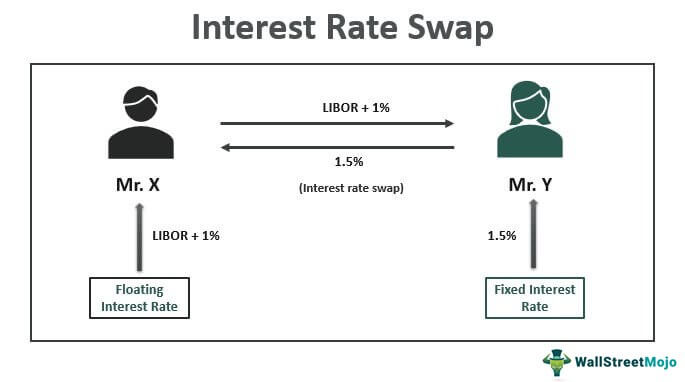
\includegraphics[width=0.9\linewidth]{Interest-Rate-Swap-diagram}
\end{center}
\end{frame}

\begin{frame}{IRS and FRA}
	\begin{itemize}
		\item We can view the last expression (\cref{eq:payoff_payer_irs}) as a portfolio of FRAs though.
		\item Indeed consider a Receiver IRS and express its payoff as a sum of FRAs with \cref{eq:fram_payoff_withF}
		\begin{equation}
			\begin{aligned}
				\textbf{RFS}&(t,T,\tau,N,K) = 	N\sum_{i=\alpha+1}^{\beta}\mathbb{E}^Q[D(t,S)\tau_i(K - L(T_{i-1},T_i))]=\\
				&=N\sum_{i=\alpha+1}^{\beta}\tau_i P(t,T_i)(K-F(t;T_{i-1},T_i))\\
				&=N\sum_{i=\alpha+1}^{\beta}\tau_i KP(t,T_i)-N\sum_{i=\alpha+1}^{\beta}(P(t,T_{i-1})-P(t,T_i)) \\
				&=N\sum_{i=\alpha+1}^{\beta}\tau_i KP(t,T_i)-NP(t,T_\alpha)+NP(t,T_\beta)
			\end{aligned}
		\label{eq:swap_as_sum_fra}
		\end{equation}
	\end{itemize}
\end{frame}

\begin{frame}{IRS and FRA}
	\begin{itemize}
		\item<1-> Clearly not all the FRAs in a swap with zero value have zero value (\emph{except for the degenerate case of flat yield curve}): some of them will have positive NPV, some other negative; the only constraint being their sum to be zero.
		\item<2-> In a \emph{Payer Swap} with an increasing yield curve the first FRAs will have negative value, the last positive. Still their NPV's sum is zero.
		\item<3-> If the market don't move so much the swap rate payer will have to pay a net interest differential in the first part of the contract life, and to receive net interest in the second.
		\item<4-> So the rate payer will have to fund the payments for the first part of the contract and to invest at his best the receipt during the second part. (This is a very hot topic nowadays; this feature is sometimes referred to as the funding profile of the contract).
	\end{itemize}
	\uncover<4->{
		\begin{tikzpicture}[remember picture,overlay]
		\node[xshift=5cm,yshift=-3.7cm] (image) at (current page.center) {
\includegraphics[width=20px]{python_logo}};
		\node[align = center, yshift=1.45cm, below=of image] {\tiny{\href{shorturl.at/xELS2}{shorturl.at/xELS2}}};
	\end{tikzpicture}}
\end{frame}

\subsection{Swap Rate}
\begin{frame}{Swap Rate as Break-Even Rate}
	\begin{block}{Definition}
	The fixed rate $K$ which makes the above expression null is called \textcolor{red}{forward swap rate}:
	\begin{equation}
		S_{\alpha,\beta}(0) = \frac{P(0, T_\alpha)-P(0,T_\beta)}{\sum_{i=\alpha+1}^{\beta}\tau_iP(0,T_i)}
	\end{equation}
	If $T_\alpha=0$ we have the \textcolor{red}{spot swap rate} (which is published on financial newspapers).
	\end{block}
	The swap rate makes the contract fair at inception by definition.
\end{frame}

\begin{frame}{Swap Payoff Alternative Expression}
	\begin{itemize}
		\item<1-> Consider a Payer IRS with $N=1$ (using \cref{eq:swap_as_sum_fra})
		\begin{equation*}
			\textbf{PFS} = P(t,T_\alpha)-P(t,T_\beta)-\sum_{i=\alpha+1}^{\beta}\tau_iKP(t,T_i)
		\end{equation*}
		\item<2-> By multiplying and dividing by (the so called \textcolor{red}{annuity}) $A = \sum_{i=\alpha+1}^{\beta}\tau_iP(t, T_i)$
		we get...
		\begin{equation}
			\begin{gathered}
			\textbf{PFS}=\frac{A}{\sum\tau_iP(t, T_i)}\left[P(t,T_\alpha)-P(t,T_\beta)-K\sum_{i=\alpha+1}^{\beta}\tau_i P(t,T_i)\right]=\\
			= A (S_{\alpha,\beta}(t)-K)
			\end{gathered}
		\label{eq:swap_payoff_with_swap_rate}
		\end{equation}
		(\textbf{note:} this expression will be useful when pricing swaptions).
	\end{itemize}
\end{frame}

\subsection{Swap and Bond Switching}
\begin{frame}{Swap and Bond Switching}
	\begin{itemize}
		\item<1-> Consider again a Payer Forward Swap (this time with notional $N$)
		\begin{equation*}
			\textbf{PFS}(t,T_\alpha,T_\beta,\tau,N,K)=N(P(t,T_\alpha)-P(t,T_\beta))-NK\sum_{i=\alpha+1}^{\beta} \tau_iP(t,T_i)
		\end{equation*}
		\item<2-> A swap can be considered as an exchange between two kinds of bond with the same notional reimbursed at maturity. In fact, \emph{the fixed leg} of the swap can be viewed as a \textcolor{red}{fixed coupon stream}, while the \emph{variable} can be considered a \textcolor{red}{floating rate note coupon stream}. 
	
%		\item When $T_\alpha = t$, i.e. we take the particular case of spot trading (PFS becomes...PS). We thus get
%		\begin{equation*}
%			\begin{aligned}
%				\text{PS}(t,T_\beta) &=N-\underbrace{NP(t,T_\beta)}_{\text{notional exch.}}-\underbrace{KN\sum_{i=\alpha+1}^{\beta} \tau_iP(t,T_i)}_{\text{coupons exch.}} \\
%				&=N-\textbf{CBP}(t,T_\beta,K,N)
%			\end{aligned}
%		\end{equation*}
	\end{itemize}
\end{frame}

\begin{frame}{Fixed Rate Side}
	\begin{itemize}
		\item<1-> More formally, consider a coupon bond that pays the following cash flows $\mathcal{C}=[c_{\alpha+1},\ldots,c_\beta]$	on the schedule $T = [T_{\alpha+1},\ldots,T_\beta]$ with 
		\begin{equation*}
			\begin{cases}
				c_i = N\tau K,\quad i<\beta \\
				c_\beta=N\tau K+N, \quad i=\beta	
			\end{cases}		
		\end{equation*}
		\item<2-> The coupon bond price can be written as the discounted sum of the cash-flows
		\begin{equation}
			\textbf{CBP}(t,\mathcal{C},T)=\sum_{i=\alpha+1}^{\beta}c_i P(t,T_i)
		\end{equation}
		\item<2-> In case $K=0$ the bond reduces to a zero-coupon bond with maturity $T_\beta$.
		
%		\item Last equation rearranged gives
%		\begin{equation}
%			\textbf{CBP}(t,T_\beta,K,N) = N - PS(t,T_\beta)
%		\end{equation}
	\end{itemize}
%	\begin{block}{Intepretation}
%		The meaning is pretty straightforward: a fixed rate bond can be replicated using the NPV of a payer swap whose fixed leg coincides with the fixed leg of the bond. The floating leg represents the funding of the bond, i.e. the interests the issuer must pay to raise funds in the interbank market when his spread over the benchmark LIBOR rate is null.
%	\end{block}
\end{frame}

%\begin{frame}{Swap and Bond Switching}
%	\begin{itemize}
%		\item More formally, consider a coupon bond that pays the following cash flows $\mathcal{C}=[c_{\alpha+1},\ldots,c_\beta]$	on the schedule $T = [T_{\alpha+1},\ldots,T_\beta]$ with 
%		\begin{equation*}
%			\begin{cases}
%			c_i = N\tau K,\quad i<\beta \\
%			c_\beta=N\tau K+N, \quad i=\beta	
%			\end{cases}		
%		\end{equation*}
%		\item The coupon bond price can be written as
%		\begin{equation}
%			\textbf{CBP}(t,\mathcal{C},T)=\sum_{i=\alpha+1}^{\beta}c_i P(t,T_i)
%		\end{equation}
%	\end{itemize}
%\end{frame}

\begin{frame}{Floating Rate Note (FRN)}
	\begin{itemize}
		\item<1-> Next consider a floating rate note that pays coupons at dates
		\begin{equation*}
			T_{\text{payments}} = [T_{\alpha+1},\ldots,T_\beta]
		\end{equation*}
		coupons calculated at the LIBOR rate fixed in the previous period
		\begin{equation*}
			T_{\text{fixings}} = [T_{\alpha},\ldots,T_{\beta - 1}]
		\end{equation*}
		\item<1-> At maturity $T_\beta$ the notional is reimbursed as before.
		\item<2-> To value the price of this note we change sign to the \textbf{RFS} (\cref{eq:swap_as_sum_fra}), set $K=0$, i.e. no fixed rate payments are done, and finally add the present value of the notional at maturity $NP(t,T_\beta)$
		\only<2-2>{\begin{equation*}
			\begin{aligned}
			\textbf{FRN} &= -\textbf{RFS} + NP(t,T_\beta) =\\
			& =NP(t,T_\alpha)-NP(t,T_\beta)-N\sum_{i=\alpha+1}^{\beta}K\tau_i P(t,T_i) + NP(t,T_\beta)
		\end{aligned}
		\end{equation*}
	    }
        \only<3->{\begin{equation*}
    		\begin{aligned}
    			\textbf{FRN} &= -\textbf{RFS} + NP(t,T_\beta) =\\
    			& =NP(t,T_\alpha)-\cancel{NP(t,T_\beta)}-\cancel{N\sum_{i=\alpha+1}^{\beta}K\tau_i P(t,T_i)} + \cancel{NP(t,T_\beta)} =NP(t,T_\alpha)
    		\end{aligned}
    	\end{equation*}
    }
	\end{itemize}
\end{frame}

\begin{frame}{Floating Rate Note (FRN)}
	\begin{itemize}
	\item The intuition behind this formula is quite straightforward: if we set $T_\alpha =t$. At the date of the first reset, the bond price equals par. 
	\item This result also holds for all the dates equal to the reset of the floating rates (an \textbf{FRN} is equivalent to a roll-over strategy of short-term loans).
	\item This property is sometimes summarized by the sentence "the \textbf{FRN} always trade at par".
	\item The \textbf{FRN} is a debt security in which coupon payments adjust according to changes in interest rates. The coupons are closely tied to current short-term spot rates, such that their prices are always at or near par value (no arbitrage). 
	%\item Provide an example of Italian government floating rate note. Did they trade at par in recent times ? Provide an explanation.
	\end{itemize}
\end{frame}

\subsection{Fixed vs Variables}
\begin{frame}{Concepts behind the Formulas}
	Suppose that a generic bank, \emph{MyFavouriteBank}, has the same credit risk of the corresponding average inter-bank entity. So, \textcolor{red}{the spread over the LIBOR rate is 0}. Suppose now the bank needs financing and it plans to issue coupon bonds. It has two alternatives:
	\begin{enumerate}
		\item<2-> borrow $N$ and pay floating interests at the rates
		\begin{equation*}
			L(T_{i-1},T_i);
		\end{equation*}
		\item<3-> borrow $N$ and pay fixed interests given by the coupon
		\begin{equation*}
			K = S_{\alpha,\beta}.
		\end{equation*}
	\end{enumerate}
\end{frame}

\begin{frame}{Concepts behind the Formulas}
	\begin{itemize}
		\item<1-> Clearly the overall cost to raise money must be the same at the beginning (fixed leg NPV equals floating leg NPV) and the bank will then opt for one of two alternatives depending on:
		\begin{enumerate}
			\item marketing considerations, i.e. which kind of bond people prefer;
			\item the interest rate risk it wants to have.
		\end{enumerate} 
		\item<2-> Remember that a variable rate mortgage is perceived risky by the average individual as salary is more or less fixed, but for bank this is not the case because it is left unarmed by the rate rise. Indeed if rates go up
		\begin{itemize}
			\item the bank loses in the higher coupons it has to pay to the bond holders;
			\item the bank gains in the highest rates it charges on new loans at the same time.
		\end{itemize}
		\item<3-> This is the most basic example of \emph{asset liability matching}.
		\item<4-> The same more or less holds for a rate decrease.%, but with some caveats.
	\end{itemize}
\end{frame}

\begin{frame}{Concepts behind the Formulas}
	\begin{itemize}
		\item Banks like floating rates exposure: 
		\begin{itemize}
			\item [\goodcheck] the liability value (the bond floating rate) resets with rates;
			\item [\goodcheck] often smaller costs then fixed rates;
			\item [\goodcheck]surely less expensive in the case of a long-term loan (e.g. 30-year mortgage), lenders require higher fixed rates in that case, due to bad accuracy in forecast economic conditions over such a long period of time.
		\end{itemize}
		\begin{itemize}
			\item [\badcheck] higher interest rate risk (risk of rising rates in the future);
			\item [\badcheck] with inverted yield curve, the cost of debt may actually be higher than fixed-rate debt (however, this is the exception rather than the norm).
		\end{itemize}
% There is a general assumption that interest rates will rise – or, increase – over time,
	\end{itemize}
\end{frame}

\begin{frame}{Concepts behind the Formulas}
	\begin{itemize}
		\item So why do not banks issue only floating rate notes ?
		\item Banks must issue fixed rate coupon bonds to attract customers (think of yourself or insurance companies) but then will hedge the liability  with an investment bank. In this way the final risk exposure will be at a variable rate as they like. 
		\item Swaps are both the hedging instrument and the pricing tool.% as formula above show.
	\end{itemize}
\end{frame}

\section{Credit Risk and Asset Swap}
\begin{frame}{Adding Credit Risk}
	\begin{itemize}
		\item When we make the real world enter the picture, a typical bank will pay a spread over LIBOR representing \textcolor{red}{credit risk} (and other stuff, but leave this extra aside for the moment). 
		%\item For the swap to be worth 0 at inception the fixed rate must be higher as well. 
		\item<2-> Hence a bank which has credit risk will have to pay
		\begin{enumerate}
			\item a higher coupon if it issues a bond with fixed coupon;
			\item a spread over the variable rate if it opts for a floating rate bond.
		\end{enumerate}
		\item<3-> Often, in the first case, it will swap the liability, i.e. the bank is liable towards the bond holders, to hedge the pure rate risk. 
		\item<4-> This lead us to the next topic, the Asset Swap (and the asset swap spread).
	\end{itemize}
\end{frame}

\begin{frame}{Par Asset Swap}
	\begin{itemize}
		\item An \textcolor{red}{Asset Swap} (AS) can be defined as a \emph{synthetic floating-rate note}.
		\item In fact, the Asset Swap transforms a fixed into a floating rate, \textcolor{red}{leaving the credit risk profile unchanged}.
		\item In the following we are going to consider \textcolor{red}{Par Asset Swaps}. 
		\item The package is made of a position in a bond and another in a swap.
		\item In case of \textcolor{red}{default} of the bond issuer, the Asset Swap buyer \textcolor{red}{must pay the fixed leg and the principal in the swap} but \textcolor{red}{does not receive the coupon} of the defaulted bond. 
	\end{itemize}
\end{frame}

\begin{frame}{Valuation of the Asset Swap}
	\begin{center}
		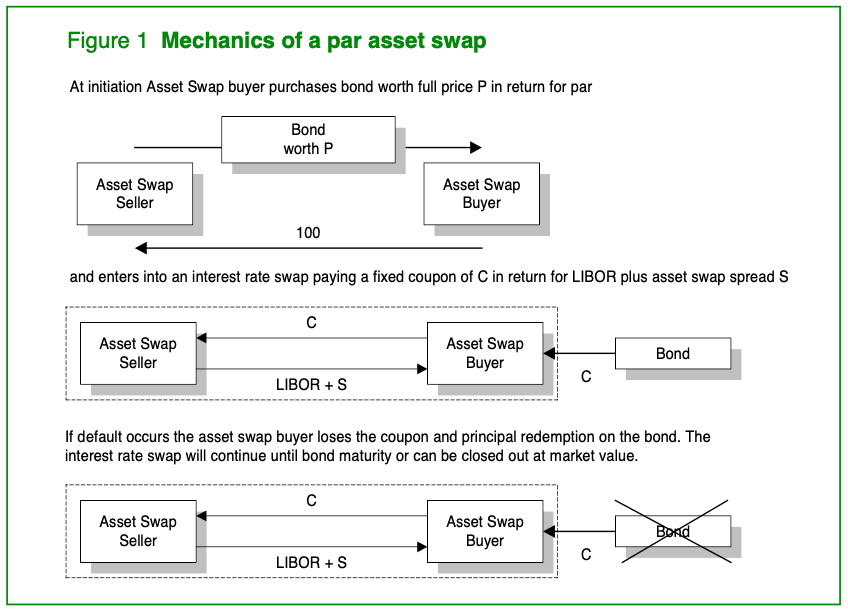
\includegraphics[width=0.7\linewidth]{asset_swap}
	\end{center}
\end{frame}

\subsection{Asset Swap Valuation}
\begin{frame}{Valuation of the Asset Swap}
	At valuation time $t$ the \emph{three} following facts are observed:
	\begin{itemize}
		\item<2-> the AS buyer buys a generic \emph{risky} coupon bond at the market price $\overline{\textbf{CBP}}(t,T,K,1)$;
		\item<3-> the AS seller pays/receives to/from the asset swap buyer the difference $\Delta = \overline{\textbf{CBP}}(t,T,K,N)-1$ in such a way that the net sum paid from the AS buyer is 1; hence \textcolor{red}{if the bond trades above par} the difference $\Delta$ is paid to the AS buyer by the seller; conversely \textcolor{red}{if the bond trades below par} the difference $\Delta$ is paid to the AS seller by the buyer.
		\item<4-> A swap is then started between the two counter-parties such that the AS seller receives a fixed leg equal to the coupon stream of the bond and the AS buyer receives the floating leg given by LIBOR rate plus a spread ($ASWS$).
	\end{itemize}
\end{frame}

\begin{frame}{Valuation of the Asset Swap}
	\begin{itemize}
		\item From the perspective of the Asset Swap seller the value of the package is given by (we are considering spot trading so $T_\alpha = t = 0$)
		\begin{equation}
			\begin{aligned}
				\textbf{ASW}=1&-\overline{\textbf{CBP}}+K\sum_{i=\alpha+1}^{\beta}\tau_i P(0,T_i)-\sum_{i=\alpha+1}^{\beta}\tau_i P(0,T_i)(L(T_{i-1},T_i)+ASWS) =\\
				=1&-\overline{\textbf{CBP}}+K\sum_{i=\alpha+1}^{\beta}\tau_i P(0,T_i)\\
				&-\sum_{i=\alpha+1}^{\beta}\tau_i P(0,T_i)L(T_{i-1},T_i)-\sum_{i=\alpha+1}^{\beta}\tau_i P(0,T_i)ASWS=0
			\end{aligned}
			\label{eq:asset_swap_value}
		\end{equation}
	\end{itemize}
\end{frame}

\begin{frame}{Valuation of the Asset Swap}
	\begin{itemize}
		\item We can replace the future rates with the forward rates, and by its definition (\cref{eq:forward_rate_definition})
		\begin{equation*}
			1 = \sum_{i=\alpha+1}^{\beta}\tau_i P(0,T_i)F(t;T_{i-1},T_i)+P(0,T_\beta)
		\end{equation*}
		hence 
		\begin{equation*}
			1 - P(0,T_\beta) = \sum_{i=\alpha+1}^{\beta}\tau_i P(0,T_i)F(t;T_{i-1},T_i)
		\end{equation*}
		\item Substitute into \cref{eq:asset_swap_value} to get
		\begin{equation*}
			\begin{aligned}
				\textbf{ASW}=1&-\overline{\textbf{CBP}}+K\sum_{i=\alpha+1}^{\beta}\tau_i P(0,T_i) -(1-P(0,T_\beta)) \\
				&+ \sum_{i=\alpha+1}^{\beta}\tau_i P(0,T_i)ASWS=0
			\end{aligned}
		\end{equation*}
	\end{itemize}
\end{frame}

\begin{frame}{Valuation of the Asset Swap}
	\begin{itemize}
		\item Canceling out the 1s
		\begin{equation*}
			\begin{aligned}
				\textbf{ASW}=&-\overline{\textbf{CBP}}+K\sum_{i=\alpha+1}^{\beta}\tau_i P(0,T_i) +P(0,T_\beta) \\
				& + \sum_{i=\alpha+1}^{\beta}\tau_i P(0,T_i)ASWS=0
			\end{aligned}
		\end{equation*}
		\item Finally we know that
		\begin{equation*}
			K\sum_{i=\alpha+1}^{\beta}\tau_i P(0,T_i) + P(0,T_\beta)
		\end{equation*}
		represents the price of coupons and principal of a bond priced off the LIBOR curve which we have assumed risk-free. We can denote it by \textbf{CBP}.
	\end{itemize}
\end{frame}
\subsection{Asset Swap Spread}
\begin{frame}{Asset Swap Spread}
	Solving for $ASWS$ we arrive at the final expression
	\begin{equation}
		ASWS = \frac{\textbf{CBP}-\overline{\textbf{CBP}}}{\sum_{i=\alpha+1}^{\beta}\tau_iP(0,T_i)}
	\end{equation}
	\begin{itemize}
	\item<2-> An asset swap enables an investor to buy a fixed rate bond and then hedge out the interest rate risk by swapping the fixed payments to floating. In doing so the investor retains the credit risk to the fixed-rate bond and earns a corresponding return. 
	\item<3-> She is still exposed to the loss of the coupons and redemption on the bond, i.e. the difference between the bond price and recovery value.
	\item<4-> In economic terms the purpose of the Asset Swap Spread is to compensate the Asset Swap buyer for taking these risks, which is measured by the spread.
	\end{itemize}
	\begin{tikzpicture}[remember picture,overlay]
	\node[xshift=5cm,yshift=-3.7cm] (image) at (current page.center) {
\includegraphics[width=20px]{python_logo}};
	\node[align = center, yshift=1.45cm, below=of image] {\tiny{\href{shorturl.at/asMU1}{shorturl.at/asMU1}}};
\end{tikzpicture}
\end{frame}

\begin{frame}{Asset Swap: Credit Considerations}
	\begin{itemize}
		\item If the credit worthiness of the issuer reduces ($\overline{\textbf{CBP}}$ decreases), rates remain constant, so $ASWS$ increases.
		\item To avoid arbitrage opportunities, $ASWS$ of bond with maturity $T_N$ must be very close to corresponding maturity CDS spread $X_N$
		\begin{itemize}
			\item if $ASWS - X_N > 0$ the investor can buy the bond, financing the purchase, enters in AS and buying protection, making an (almost) risk free profit (\emph{negative basis trading});
			\item if $ASWS - X_N < 0$ can do the opposite.
		\end{itemize}
		%If the bond defaults, the asset swap buyer has to continue paying on the swap — which can no longer be funded with the coupon from the bond — or the swap can be closed out at market value. The asset swap buyer also loses the par redemption of the bond, receiving whatever recovery rate the bond issuer pays. 
		\item Since the $ASWS$ is quoted as a spread to LIBOR, for assets of better credit quality than AA-rated banks it may be negative.
	\end{itemize}
\end{frame}

\subsection{Delta Measures}

\begin{frame}{Delta Risk}
	\begin{itemize}
	\item The concept of delta risk on interest rate derivatives is a generalization of the traditional one of a single asset option. 
	\item However fixed income derivatives depend on a variety of
	instruments, used in the determination of the interest rate curve, rather than a single asset.
	\item The delta risk measures precisely the risk associated with the
	shift of the interest rate curve. 
	\item Because there are many ways of shifting the interest rate curve, many different deltas can be computed. 
	\end{itemize}
\end{frame}

\begin{frame}{Swap Delta Measures}
	\begin{itemize}
		\item \textbf{Basis Point Value:} the variation (in EUR) of the swap $NPV$ in response to a 1 bp change in yields all along the yield curve (parallel shift in the yield curve). It is equal to the discounted value of the cash-flows for a rate of 0.01\% for all periods of the fixed leg with a rate of 0.01
		\begin{equation}
			BPV(t,T_\beta) = 0.01\%\sum_{i=\alpha+1}^{\beta}\tau_iP(0,T_i);
		\end{equation}
		\item \textbf{Modified Duration:} is the relative variation of a bond price given the variation of the reference rate. Since swaps can be thought of exchange of two bonds it can be used as a delta measure as well.
	\end{itemize}
	\begin{tikzpicture}[remember picture,overlay]
	\node[xshift=5cm,yshift=-3.7cm] (image) at (current page.center) {
\includegraphics[width=20px]{python_logo}};
	\node[align = center, yshift=1.45cm, below=of image] {\tiny{\href{shorturl.at/mqvFP}{shorturl.at/mqvFP}}};
\end{tikzpicture}
\end{frame}

\begin{frame}{Swap Delta Measures}
	\begin{itemize}
		\item \textbf{Market Rate Sensitivity:} it is given by the sum of the swap $NPV$ variations obtained by shifting one by one, by a bps, the input market instruments used in the yield curve bootstrap. In a plain vanilla swap is very close but not equal to BPV.
		\item The mark to market value of the swap is \textcolor{red}{not linear} (as in a future contract), but rather it is a \textcolor{red}{convex} function of the rates (just like a bond is a convex function of the yield).
		\begin{columns}
		\column{0.45\linewidth}
		\item If interest rates go down, the swap’s profit is more than proportional, whilst if rates go up, the loss is also more than proportional.
		\begin{equation*}
			\frac{\Delta P}{P}\approx -D \Delta y
		\end{equation*}
		%\item This is the reason why $BPV$ and sensitivity are not exactly the same number.
		\column{0.45\linewidth}
		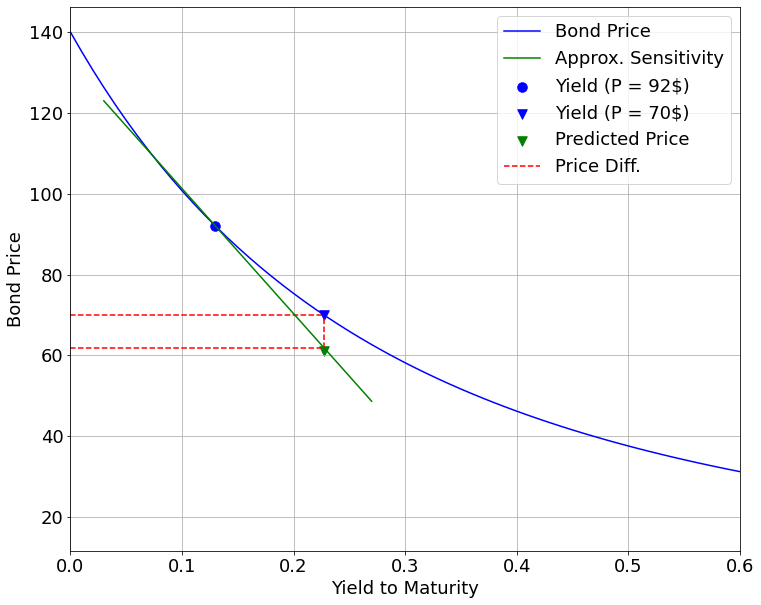
\includegraphics[width=0.8\linewidth]{bond_duration}
		\end{columns}
%		\item Suppose for instance that we are short on a five year swap and to receive $4y$. If the rates go higher we lose money, but the rate of variation of the MTM decreases with the increases of rates. If rates decrease, the MTM increases, and the rate of variation of the MTM increase with the further increase with the further decrease of rates.
	\end{itemize}
\end{frame}

%\begin{frame}{Considerations}
%	\begin{itemize}
%		\item Higher rates affect the $NPV$ in two ways: via the discounting and via the forecasting. If the rates go higher the present value of both legs is lower, but the forecasted value of the floating leg is higher: forward rates are higher.
%		\item The way the curve is bootstrapped interferes with the calculation of the delta also for bullet swaps especially in the front end because the curve is bootstrapped using different instruments.
%	\end{itemize}
%\end{frame}

\begin{frame}{Trading and Hedging Swaps}
	\begin{itemize}
		\item With a swap you can have a clear picture of the market. For example if you own the $5y$, you make money if rates go higher, loose money if they go lower.
		\item With two swaps instead you can bet on the \textcolor{red}{slope} of the interest rate curve.
		\item If you bet on steepening of the $30y-10y$ slope, you pay the $10y-30y$; if you bet on flattening on the same portion of the yield curve you receive the $10y-30y$.		
		\item With swaps you can bet on the \emph{bund basis}: this quantity is linked to the evolution of credit and liquidity in the inter-bank and Government bond markets.
	\end{itemize}
\end{frame}

%\begin{frame}{Trading and Hedging Swaps}
%	For example, the yield spread is 0.6524\%. An investor believes that this yield spread will narrow as inter-bank credit improves relative to German Sovereign credit. By entering into a position which profits from a rise in the lower (German	Sovereign) yields and / or a fall in the higher (inter-bank) yields, the investor is able to express his view on relative credit pricing.
%	AGGIUNGERE UN PO' DI SPIEGAZIONE
%\end{frame}

\section{Cap and Floor}
\begin{frame}{Caps and Floors}
	\begin{itemize}
		\item<1-> A \textcolor{red}{Cap} is a Payer IRS in which the payment is done only if the payoff is positive. Its value is the expectation of 
		\begin{equation}
			\sum_{i=\alpha+1}^{\beta}D(t,T_i)N\tau_i\max\left[L(T_{i-1},T_i)-K,0\right]
			\label{eq:cap}
		\end{equation} 
		\item<1-> The cap allows investors which have a debt at a variable rate to buy insurance against high rates in the future.
	
		\item<2-> A \textcolor{red}{Floor} is the same kind of object but analogous to a Receiver IRS:
		\begin{equation}
			\sum_{i=\alpha+1}^{\beta}D(t,T_i)N\tau_i\max\left[K-L(T_{i-1},T_i),0\right]
			\label{eq:floor}
		\end{equation} 
	\end{itemize}
\end{frame}

\subsection{Caplets}
\begin{frame}{Caplet and Floorlet}
	\begin{itemize}
		\item<1-> Considering each element of the sum in \cref{eq:cap} or \cref{eq:floor} we see that Cap/Floor can be split into forward starting options over a floating rate, called \textcolor{red}{Caplet/Floorlet}.
		\item<2-> A Caplet/Floorlet payoff is defined as
		\begin{equation*}
			D(t,T_i)N\tau_i\max\left[L(T_{i-1},T_i)-K,0\right]
		\end{equation*} 
		and its value is given by
		\begin{equation}
			\textbf{Cpl}(t,T_{i-1},T_i,\tau,N,K)=\mathbb{E}^{\mathcal{Q}}\left(e^{-\int_t^{T_i}r_s ds}N\tau(L(T_{i-1},T_i)-K)^+ | \mathcal{F}_t\right)
		\end{equation}
		\item This can also be written
		\begin{equation*}
			\textbf{Cpl}=N\mathbb{E}^{\mathcal{Q}}\left(e^{-\int_t^{T_{i-1}}r_s ds}\tau P(T_{i-1},T_i)(L(T_{i-1},T_i)-K)^+ | \mathcal{F}_t\right)
		\end{equation*}
	\end{itemize}
\end{frame}

\begin{frame}{Caplets as ZCB Put Options}
	\begin{itemize}
		\item<1-> Using the LIBOR rate definition we get
		\begin{equation*}
			\begin{aligned}
				\textbf{Cpl} &=N\mathbb{E}^{\mathcal{Q}}\left(e^{-\int_t^{T_{i-1}}r_s ds}P(T_{i-1},T_i)\left[\frac{1}{P(T_{i-1},T_i)}-1-K\tau\right]^+ | \mathcal{F}_t\right) \\
				& = 		N\mathbb{E}^{\mathcal{Q}}\left(e^{-\int_t^{T_{i-1}}r_s ds}\left[1-(1+K\tau)P(T_{i-1},T_i)\right]^+ | \mathcal{F}_t\right)
			\end{aligned}
		\end{equation*}
		\item<2-> Multiplying by $\frac{1}{1+K\tau}$ we finally get
		\begin{equation}
			\textbf{Cpl}=N(1+K\tau)\mathbb{E}^{\mathcal{Q}}\left(e^{-\int_t^{T_{i-1}}r_s ds}\left[\frac{1}{1+K\tau}-P(T_{i-1},T_i)\right]^+ | \mathcal{F}_t\right)
		\end{equation}
	\end{itemize}
\end{frame}

\begin{frame}{Caplets as ZCB Put Options}
	\begin{block}{Intepretation}
		Caplets can then be seen as \textcolor{red}{put options} on ZCBs. In the same way, floorlets can be seen as \textcolor{red}{call options} on ZCBs.
	\end{block}
\end{frame}

\section{The Black Model}
\begin{frame}{The Black Model - Overview}
	\begin{itemize}
		\item The \textcolor{red}{Black Model} extends the Black-Scholes formula to \emph{caplets}, \emph{swaptions} and \emph{bond option prices}. %It uses the forward coordinates, not the spot ones; this last is not a minor issue indeed.
		\item The main difference with respect to the Black-Scholes set up is that \textcolor{red}{forward rates are log-normally distributed}, rather than the spot price of the underlying.
		\item So $F(t;T_{i-1},T_i)$ (or $S_\alpha(t)$) are modeled as log-normal random variables. 
		
		\textcolor{red}{But not at the same time !} If $F(t;T_{i-1},T_i)$ is log-normal, then $S_\alpha(t)$ cannot be.
		
		%\item Alert: if LIBOR/EURIBOR simple rates are log-normal, swap rates cannot be. This theoretical inconsistency is negligible in real world situations.
	\end{itemize}
\end{frame}

%\begin{frame}{The Black Model: Overview}
%	\begin{itemize}
	%		\item It should be recognized that the Black model is being actually used in different ways. In particular the caps uses the forward short-term LIBOR rate as the underlying state variable, whereas the swaptions uses longer-term forward swap rates. Beause forward swap rates are nearly linera in individual forward rates , the lognormality assumption implicit in the Black model cannot hold simultaneously for both, since a linear combination of lognormal variables is not lognormal.
	%	\end{itemize}
%\end{frame}

\begin{frame}{The Black Model: Overview}
	\begin{itemize}
		\item It is widely used in practice. 
		\item Black formula was indeed the metric by which traders translated volatilities into prices until rates became too low and the model collapsed under the assumption of positive rates.
		\item ...but for the moment we cannot consider it as a model ! Just a bunch of formulas.
		
		Their formal justification will be provided later in the context of the \textcolor{red}{Libor Market Model}.
	\end{itemize}
\end{frame}

\begin{frame}{Pricing Caps with the Black-76 Formula}
	\begin{block}{Definition}
	\begin{equation}
		\begin{aligned}
		\textbf{Cap}_{Bl}(0, \tau,N,K,\sigma_{\alpha,\beta}) &= 		N\sum_{i=\alpha+1}^{\beta} \textbf{Caplet}_{Bl}(T_i, \tau,K,\sigma_{\alpha,\beta}) = \\ &=N\sum_{i=\alpha+1}^{\beta}P(0,T_i)\tau Bl(K,F(0;T_{i-1},T_i),v_i)
		\end{aligned}
		\label{eq:cap_black}
	\end{equation}
	where
	\begin{equation*}
		\begin{gathered}
			Bl(K,F,v)=F\Phi(d_1(K,F,v)) - K\Phi(d_2(K,F,v)) \\
			d_{1,2} = \frac{\log{\cfrac{F}{K}} \pm \cfrac{v^2}{2}}{2} \\[0.2cm]
			v_i = \sigma_{\alpha,\beta}\sqrt{T_{i-1}}	
		\end{gathered}
	\end{equation*}
	\end{block}
\end{frame}

\subsection{Cap/Floor Volatility}
\begin{frame}{Flat and Spot Volatilities}
	\begin{itemize}
		\item When comparing to other vanilla derivatives, Cap/Floor pricing offers an additional complexity, as it does not involve a single volatility number. 
		\item As seen Cap/Floor can be \textcolor{red}{stripped} into Caplet/Floorlet which should be priced with a different volatility each. 
		\item However, Caplet/Floorlet volatilities (\textcolor{red}{spot volatilities}) are not quoted directly on the market.
		\item The market instead quotes Cap/Floor $\sigma_{\alpha,\beta}$, i.e. \textcolor{red}{flat volatilities}, typically for a range of strikes and expiries over liquid floating rates (e.g. 3M and 6M Euribor).
		\item Although being quoted, \textcolor{red}{flat volatilities have little financial meaning}. Conversely spot volatilities cannot be observed directly but are the quantities \textcolor{red}{naturally tied to forward rates as a measure of their uncertainty}.
	\end{itemize}
\end{frame}

\begin{frame}{Main Challenges}
	\begin{enumerate}
		\item Produce Caplet/Floorlet prices consistent with current levels of Cap/Floor volatilities and therefore be able to re-price the market;
		\item being able to “rebase” volatilities when pricing Cap/Floor over not quoted floating rates according to multiple curves framework (e.g. Cap/Floor over 1M or 12M Euribor);
		\item to make things more complicated, some Caps/Floors are not always quoted over the same LIBOR, for example EUR Cap/Floor are quoted over 3M EURIBOR up to $2y$ maturity and then over 6M EURIBOR.
	\end{enumerate}
	\begin{tikzpicture}[remember picture,overlay]
		\node[xshift=5cm,yshift=-3.7cm] (image) at (current page.center) {
\includegraphics[width=20px]{python_logo}};
		\node[align = center, yshift=1.45cm, below=of image] {\tiny{\href{shorturl.at/ekDGM}{shorturl.at/ekDGM}}};
	\end{tikzpicture}
\end{frame}
%
%\begin{frame}{Bootstrapping Caplet Volatilities}
%	\begin{itemize}
	%		\item From the prices of different maturity caps, it is possible to \textcolor{red}{bootstrap} the volatility of each caplet, i.e. the volatility which refers to the forward rate corresponding to the caplet.
	%		\item Let’s take a concrete example; we would like to price a $3y$ Cap with 0.5\% strike over $6m$ EURIBOR. We will have to price 6 Caplets hence we will need 6 different volatilities.
	%		\item Few assumptions:
	%		\begin{itemize}
		%			\item we have volatilities for the 0.5\% strike for maturities $1y$, $18m$, $2y$ and $3y$ (this is generally the case for EUR);
		%			\item the volatility is a piecewise constant function of time, i.e. that it is constant between two quoted points;
		%			\item we start with the nearest instruments, i.e. the spot starting caplet with $6m$ maturity, since the volatility is constant between spot and $1y$, it will be priced with the $1y$ volatility such as:
		%			\begin{equation*}
			%			\sigma_{caplet}(0.5,t_{0,6m})=\sigma_{Cap}(0.5,t_{0,1y})
			%			\end{equation*}
		%		\end{itemize}
	%	\end{itemize}
%\end{frame}
%
%\begin{frame}{Bootstrapping Caplet Volatilities}
%	\begin{itemize}
	%		\item Let’s now price the $1y$ forward starting caplet with $6m$ maturity. We assumed the $18m$ volatility is quoted. Since market  Cap volatilities are quoted assuming no-arbitrage opportunity we can build the forward starting caplet as the difference of the two:
	%		\begin{equation*}
		%			Cpl(1y, 1y6m)=Cap(1y,6m)-Cap(1y)
		%		\end{equation*}
	%		\item Previous equation will yield a premium and then we will be able to solve a single volatility for such premium by using a Newton-Raphson or bisection method.
	%		\item We can apply the same method for the $1y6m$ forward starting caplet to get the volatility.
	%	\end{itemize}
%\end{frame}
%
%\begin{frame}{Bootstrapping Caplet Volatilities}
%	\begin{itemize}
	%		\item We can now move to the $2y$ forward starting caplet. The main issue here is that we do not have $2y6m$ Cap volatility quoted on the market, so we are assuming for the sake of simplicity that the volatility remains constant between $2y$ and $3y$ Caps. Therefore we will use the following formula:
	%		\begin{equation*}
		%			Cpl(2y, 2y6m)=Cap(2y,6m)-Cap(2y)
		%		\end{equation*}
	%		With $\sigma_{Cap}(0.5,t_{0,2y6m})=\sigma_{Cap}(0.5,t_{0,3y})$. (We could also use an interpolation method such as linear or cubic spline to get the $2y6m$ Cap volatility.
	%		\item Finally we solve the $2y$ forward starting caplet volatility as previously and ultimately we can compute the last caplet ($2y6m$ forward starting) following the same method.
	%	\end{itemize}
%\end{frame}
%
%\begin{frame}{Remarks on Bootstrapping}
%	\begin{itemize}
	%	\item In some situations the forward starting caplet’s premium can be negative or too low to solve the caplet volatility. Typically it can occur when using a different basis (i.e. LIBOR tenor) when switching from one Cap to another. 
	%	%(especially when using Black volatilities where volatilities on shorter basis can be much higher than longer basis).
	%	%In our example Caps are quoted over 3M Euribor for 1Y, 18M and 2Y maturities and then over 6M Euribor. When using directly 3M Euribor Cap volatilities to price a 6M Euribor Cap without any adjustments we assume implicitly that 3M Volatilities are following the same dynamic as 6M (i.e. that they trade with a 100% correlation). This is actually an assumption implying that the curve will be only subject to parallel moves, ruling out any possibility of curve steepening.
	%	\item Obviously the piecewise constant interpolation method can lead to some local arbitrage opportunities (on an interpolated caplet), when using a different method we can see that we will get a different volatility, the only constraint being repricing “globally” the cap through the 1-dimensional solver.
	%	\end{itemize}
%\end{frame}

%\item These parameters are then used for pricing under the assumption of log-normal forward rates. These are called \textcolor{red}{spot volatilities}.
%\item Notice that the smile is neglected in this model.


%\item Indeed in the market a surface of implied volatility is quoted: a volatility for each standard maturity and for several strikes. This is in contrast with the assumption of log-normality: changing volatility seems an abuse of the concept of model.
%\item As someone put it: implied volatility is the wrong number in the wrong model to get the (right) market price (Rebonato).
%	\end{itemize}
%\end{frame}

%\begin{frame}{What you find in the market}
%	\begin{itemize}
%		\item Standard caps are quoted with euribor-3m as the underling and 3m caplets for maturities [1y-18m-2y] and with euribor-6m as the underlying and 6m caplets for maturities [3y-30y].
%		\item Strikes range from -0.757\% to 10\%.
%	\end{itemize}
%\end{frame}

%\begin{frame}{Flat and Spot Volatilities}
%	\begin{itemize}
%		\item The market quotes cap volatilities for at-the-money options and several other strikes (the smile).
%		\item Cap volatilities are known as \emph{flat} volatilities, while caplet volatilities must be bootstrapped and are known as \emph{spot} volatilities.
%
%		\item There is a sort of inconsistency in this market practice. The same caplet belonging to two different caps, even if refers to the same time period, is being valued using different volatilities...
%		\item and the different caplets of the same cap share the same volatility.
%		\item Bootstrapping is the way to solve the puzzle.
%	\end{itemize}
%\end{frame}

\begin{frame}{Problems with the Black Model}
\begin{itemize}
	\item In the Black model \textcolor{red}{negative rates are not allowed}. Hence a zero strike floor cannot be priced
	\begin{equation*}
		d_{1,2} = \frac{\boxed{\log{\frac{F}{K}}} \pm \cfrac{v^2}{2}}{2} 
	\end{equation*}
	but in the last years in the inter-bank market it is not so unusual to find prices for -1\% strike floors.
	\item Moreover in the Black model the empirical evidence of the smile is not accounted for (i.e. $\sigma$ is a constant). Two caps identical but for the strike need a different volatility to recover two different market prices if one uses Black formula.
	%\item And this is clear if one looks at the distribution and at the process of $F(t, T, S)$; the volatility does not depend on the strike of the option. It is a characteristic of the forward rate.
\end{itemize}
\end{frame}

\begin{frame}{The Practitioner Solutions}
\begin{itemize}
	\item To face the smile, the model is used with \textcolor{red}{different input volatilities for different strikes}. In practice the model is a mapping of implied volatilities into prices and viceversa%, and it is used to bootstrap caplet volatilities which have a financial meaning, while cap volatilities have not.
	\item To face the non negative rates, Black model has been \textcolor{red}{shifted}. The technique was already known but in the last years has become crucial to shift the lower bound of prices admitted by the model.
\end{itemize}
\end{frame}

\begin{frame}{Shifted Lognormal Model for Caplets}
\begin{itemize}
	\item It can be shown that Black formula provides valid solutions if strike and forward rate are \textcolor{red}{shifted}. For a $(T,S)$ caplet with strike $K$ we get
	\begin{equation}
		\textbf{Caplet}_{Bl}(t,T,S,\tau,K,v_T,\alpha) = P(t,S) Bl(K-\alpha,F(t;T,S)-\alpha,v_T)
	\end{equation}
	where $d_1$ and $d_2$ read as before and instead $v_i$ is now given by
	\begin{equation*}
		v_T = \sigma^{\text{shifted}}\sqrt{T}
	\end{equation*}
	\item The market quotes of $\sigma^{\text{shifted}}$ refer to shifts $\alpha$ of the order of [2\%,3\%].
	%\item What is the relationship between $\sigma^{\text{shifted}}$ and $v_T$ ?
	%\item Rewrite the Black-76 SDE for the $(T, S)$ caplet as follows
	%\begin{equation}
	%	dF(t,T,S)=\sigma^{\text{shifted}}(F(t,T,S)-\alpha)dW^{\mathcal{Q}_S}(t)
	%\end{equation}
	%\item It is easy to see that the price for a $(T,S)$ caplet with strike $K$ is given by
	%\begin{equation}
	%	Cpl(t,T,S,\tau,K,v_T,\alpha)=P(t,S)Bl(K-\alpha,F(t,T,S)-\alpha,v_T)
	%\end{equation}
\end{itemize}
\end{frame}

%\begin{frame}{Shifted Lognormal Model for Caplets}
%	\begin{itemize}
%		\item Where $d_1$ and $d_2$ read as before and instead $v_i$ is now given by
%		\begin{equation}
	%			v_T = \sigma^{\text{shifted}}_{\alpha,\beta}\sqrt{T}
	%		\end{equation}
%		\item In the market $\sigma^{\text{shifted}}_{\alpha,\beta}$ is quoted (with $\alpha \in [2\%,3\%]$).
%		\item What is the relationship between $\sigma^{\text{shifted}}$ and $v_T$ ?
%	\end{itemize}
%\end{frame}

\begin{frame}{The Volatility Hump}
\begin{itemize}
	\item Empirical studies have pointed out two very important issues:
	\begin{itemize}
		\item the first one is that interest rates volatility can depend on the level of the interest rates themselves;
		\item moreover the volatility function is increasing in the short end of the curve, and decreasing in the long end, with an \textcolor{red}{humped} type movement.
	\end{itemize}  
	\begin{columns}
		\column{0.45\linewidth}
		\item Uncertainty is bigger in the intermediate region and lower in the front of the maturity spectrum. For long maturities volatility tends to decay.
		\item When the hump does not appear it is regarded as \emph{stressed market}.
		%\item There is a financial explanation for this feature.
		\column{0.45\linewidth}
		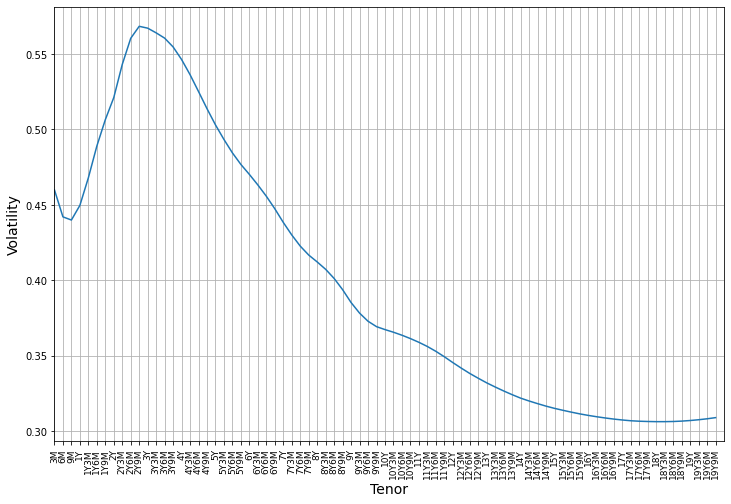
\includegraphics[width=1.1\linewidth]{cap_vola}
	\end{columns}
\end{itemize}
\end{frame}

\section{Swaptions}
\begin{frame}{Swaptions Overview}
\begin{itemize}
	\item There are two main types of \textcolor{red}{swaptions} (as the underlying swaps), a \emph{payer} and a \emph{receiver} version.
	\item In an \textcolor{red}{European payer swaption}, the purchaser has the right but not the obligation to enter into a swap contract, at a given future time, called the \textcolor{red}{swaption maturity},	where they become the fixed-rate payer and the floating-rate receiver (a receiver swaption is the opposite). 
	\item A swaption provides protection for a borrower as it ensures a maximum fixed interest rate payable in the future. Furthermore, it gives the borrower flexibility, if the rate does not rise to the swaption strike rate at expiry the borrower can choose not to exercise it and tak advantage of the lower market rates.
\end{itemize}
\end{frame}

\begin{frame}{Swaptions Overview}
	\begin{itemize}
	\item Usually, the swaption maturity coincides with the first reset date of the underlying IRS.
	\item The length of the underlying IRS is called the \textcolor{red}{tenor} of the swaption.	
	\item If you are on the buyer side (you are long payer swaption) which is your view on rates ? Why ? And the receiver ?
\end{itemize}
\end{frame}

\begin{frame}{Swaption Payoff}
\begin{itemize}
	\item The discounted payoff of a payer swaption (with maturity $T_\alpha$) is given, recalling the value of a payer IRS ($
	\sum_{i=\alpha+1}^\beta P(T_\alpha,T_i)\tau_i (F(T_\alpha;T_{i-1},T_i) - K)$)
	by
	\begin{equation}
		\textbf{PS}=D(t,T_\alpha)\left(\sum_{i=\alpha+1}^\beta P(T_\alpha,T_i)\tau_i (F(T_\alpha;T_{i-1},T_i) - K)\right)^+
	\end{equation}
	\item This payoff cannot be easily decomposed in elementary parts (as done for Cap/Floor). Indeed the \emph{positive part operator} $(\cdot)^+$ is "outside" the summation (while for Cap it is "inside").
	\item Nevertheless it can be rewritten in a different way.
	%		\begin{equation}
		%			ND(t,T_\alpha)\left(S_{\alpha,\beta}(T_\alpha)-K\right)^+\sum_{i=\alpha+1}^\beta \tau_i P(t,T_i)
		%		\end{equation}
\end{itemize}
\end{frame}

\begin{frame}{Swaption Payoff}
\begin{itemize}
	\item<1-> Recall that we have expressed the swap payoff also as (\cref{eq:swap_payoff_with_swap_rate})
	\begin{equation*}
	\textbf{PFS}=\sum_{i=\alpha+1}^\beta \tau_i P(t,T_i)(S_{\alpha,\beta}-K)
	\end{equation*}
	\item<2-> If we look at the swaption payoff in this way and we model directly $S_{\alpha,\beta}(t)$ instead of $F(t;T_{i-1},T_i)$ we can write the swaption price as the expectation of the following expression
	\begin{equation}
		\textbf{PS}=\left[D(t,T_\alpha)A\max(S_{\alpha,\beta}(T_\alpha)-K, 0)\right]
	\end{equation}
	which looks like easier and more intuitive than the previous expression.
\end{itemize}
\end{frame}

\begin{frame}{Swaption Characterization}
	\begin{itemize}	
		\item We characterize the payoff in three different ways
		\begin{enumerate}
			\item The swaption is said to be \textcolor{red}{at-the-money} (ATM) if
			\begin{equation*}
				K = K_{ATM} = S_{\alpha,\beta}(0) = \frac{P(0,T_\alpha)-P(0,T_\beta)}{\sum_{i=\alpha+1}^\beta \tau_i P(0,T_i)}
			\end{equation*}
			where $T_\alpha$ is the maturity of the swaption, and $T_\beta$ the last payment date of the underlying swap (the first being $T_{\alpha+1})$. That is when the strike is equal to the swap forward rate $S_{\alpha,\beta}$.
			\item The payer swaption is \textcolor{red}{in-the-money} if $K<K_{ATM}$ and \textcolor{red}{out-of-the-money} otherwise.
			\item The opposite holds for the receiver swaption.
		\end{enumerate}
		\item ATM swaptions are quoted for maturities ranging between $1m$ and $30y$, and for tenors between $1y$ and $30y$.
	\end{itemize}
\end{frame}

%\begin{frame}{Swaption as an Option on a Swap}
%	\begin{itemize}
%		\item So the forward rates are the chosen state variable, also the correlation between them is needed...
%		\item Market practice: approximation formula (see chapter 6 of Brigo-Mercurio) the definitive reference for this issue.
%		\item Clearly here a model which accounts for terminal correlations needed.
%		\item Which is the relationship between a Cap and a payer swaption with the same payment and roll dates ?
%	\end{itemize}
%
%\end{frame}

\begin{frame}{An Example}
	\begin{itemize}
		\item \textbf{A} has raised a $10y$ loan with floating interest rates fixed every three months (IBOR + margin).
		\item \textbf{A} wants to \emph{hedge the loan against rising interest rates but also to benefit from the floating rate}, i.e. should fixed interest rates not rise above a certain level (the swaptions strike-rate $K$).
		\item The purchase of a payer swaption could hedge this risk: 
		\begin{columns}
			\column{0.45\linewidth}
			\begin{itemize}
				\item \textbf{interest rates increase}: \textbf{A} may exercise the swaption and be a party of a swap as a payer of a fixed interest rate;
				\item \textbf{swap-rate below $K$}: it will not be exercised and \textbf{A} will continue to have floating-rate funding.
			\end{itemize}
			\column{0.45\linewidth}
			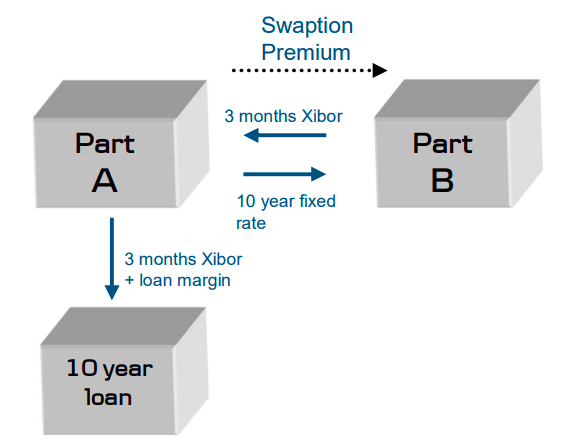
\includegraphics[width=1.\linewidth]{swaption_example}
		\end{columns}
	\end{itemize}
\end{frame}

\begin{frame}{Differences between Caps and Swaptions}
\begin{itemize}
	\item As we have seen caps can be decomposed into more elementary products: \textcolor{red}{caplets}. You can simply value each caplet at once and then add their prices
	\begin{itemize}
		\item you can value them modeling each forward rate at once;
		\item \textbf{no joint action of forward LIBOR rates is involved.}
	\end{itemize}
	\item Unfortunately this is not possible in swaptions.
	\item The swap rate is \textcolor{red}{almost a weighted average of forward rates} $S=\cfrac{\sum F(t;T_{i-1},T_i)}{\sum P(t,T_i)}$, hence its volatility should depend on the forward rate volatilities as well as their correlations.
	\item if you take as "fundamental" entity the LIBOR rates you have to deal with the joint action of the simple forward LIBOR rates and so with the \textbf{terminal correlation} between rates of different portions of the yield curve. 
	%Can you provide an example ?
\end{itemize}
\end{frame}

\subsection{Bond Options}
\begin{frame}{An Option to Exchange Fixed with Float}
\begin{itemize}
	\item We have seen that a Swap can be viewed as an exchange of bonds (fixed for float).
	\item Hence a Swaption can be regarded as an \textcolor{red}{option to exchange fixed for floating} bonds (or viceversa).
	\item To fully characterized this point we need an expression for a \textcolor{red}{Coupon Bond Option}.
	\item Most interest rate models have closed formulas for the Zero Coupon Bond price. So it would be a great simplification if we could express a Coupon Bond Option as a portfolio of Zero Coupon Bond Options.
	\item Luckily we can do that thanks to a recipe known as \textcolor{red}{Jamshidian's decomposition}.
\end{itemize}
\end{frame}

\begin{frame}{Jamshidian's Trick}
\begin{block}{Theorem}
	Consider a sequence of functions $f_i$, a random variable $W$ and a constant $K\ge0$. If each $f_i$ is monotone (decreasing), that is $\cfrac{\partial f_i}{\partial W} < 0;\;\forall i$, then 
	\begin{equation*}
		\left(K - \sum_i f_i(W)\right)^+ = 	\sum_i \left(K_i - f_i(W)\right)^+
	\end{equation*} 
	In financial terms it means that the payoff of an option on a portfolio of assets can be expressed in terms of a portfolio of options on each asset.
\end{block}
\end{frame}

\begin{frame}{Jamshidian's Trick Proof}
\begin{itemize}
	\item Since $\sum_i f_i$ is also monotone decreasing there is a unique solution $\hat{w}$ to 
	\begin{equation*}
		\sum_i f_i(\hat{w}) = K
	\end{equation*}
	\item<2-> Finally since each $f_i$ is decreasing
	\begin{columns}
	\column{0.7\linewidth}
	\only<2-2>{\begin{equation*}
		\begin{aligned}
			&\left(K - \sum_i f_i(W)\right)^+ = \left(\sum_i f_i(\hat{w}) -  \sum_i f_i(W)\right)^+ 
		\end{aligned}
	\end{equation*}}
	\only<3-3>{\begin{equation*}
		\begin{aligned}
			&\left(K - \sum_i f_i(W)\right)^+ = \left(\sum_i f_i(\hat{w}) -  \sum_i f_i(W)\right)^+ = \\ 
			& = \left(\sum_i (f_i(\hat{w}) -  f_i(W))\right)^+
		\end{aligned}
\end{equation*}}
	\only<4-4>{\begin{equation*}
		\begin{aligned}
			&\left(K - \sum_i f_i(W)\right)^+ = \left(\sum_i f_i(\hat{w}) -  \sum_i f_i(W)\right)^+ = \\ 
			& = \left(\sum_i (f_i(\hat{w}) -  f_i(W))\right)^+= \sum_i (f_i(\hat{w}) - f_i(W))\mathbb{1}_{W\le \hat{w}}
		\end{aligned}
\end{equation*}}
	\only<5-5>{\begin{equation*}
		\begin{aligned}
			&\left(K - \sum_i f_i(W)\right)^+ = \left(\sum_i f_i(\hat{w}) -  \sum_i f_i(W)\right)^+ = \\ 
			& = \left(\sum_i (f_i(\hat{w}) -  f_i(W))\right)^+= \sum_i (f_i(\hat{w}) - f_i(W))\mathbb{1}_{W\le \hat{w}} = \\ 
			&= \sum_i \left(K_i - f_i(W)\right)^+
		\end{aligned}
\end{equation*}}
	\column{0.35\linewidth}
	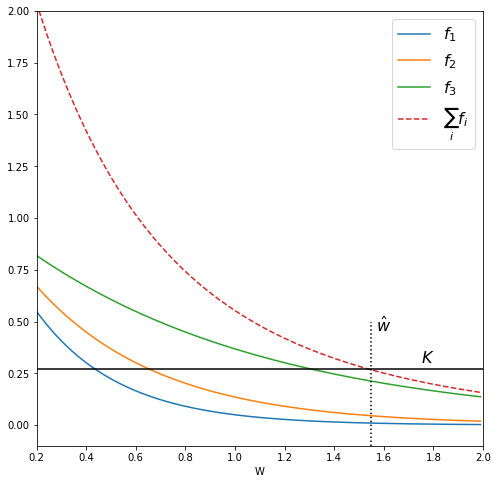
\includegraphics[width=1\linewidth]{jamshidian_trick}
	\end{columns}
\end{itemize}
\end{frame}

\begin{frame}{Back to Coupon Bond Option}
\begin{itemize}
	\item Consider a coupon bond which pays the following cash flows $\mathcal{C}=\{c_1,\dots,c_n\}$ at dates $T=\{T_1,\ldots,T_n\}$.
	\item Let $t\leq T_1$, the bond price is given by
	\begin{equation*}
		\textbf{CB}(t,\mathcal{C},T)=\sum_{i=1}^n c_i \Pi(t, T_i, r(t))
	\end{equation*}
	\item Suppose we would like to calculate the price of a put option with strike $K$ on this coupon bond. The payoff reads
	\begin{equation*}
		\textbf{CBP}=\left[K-\textbf{CB}(t,\mathcal{C},T)\right]^+ = \left[K-\sum_{i=1}^n c_i \Pi(t, T_i, r(t))\right]^+
	\end{equation*}
\end{itemize}
\end{frame}

\begin{frame}{Coupon Bond Option}
\begin{itemize}
	\item Now apply the Jamshidian's decomposition to the previous payoff.
	\item So first need to find the interest rate value $r^*$ such that $\sum_{i=1}^n c_i \Pi(t, T_i, r^*) = K$.
	\item Assuming the interest rate model satisfies the required condition
	\begin{equation*}
		\frac{\partial \Pi(t,T_i,r(t))}{\partial r}<0,\;\forall 0<t<s
	\end{equation*}
	we can rewrite the payoff as
	\begin{equation}
		\textbf{ZBP}(t,T_i,\Pi,r^*) = \sum_{i=1}^n c_i [\Pi(t, T_i, r^*)-\Pi(t, T_i, r(t))]^+
	\label{eq:bond_option_payoff}
	\end{equation}
\end{itemize}
\end{frame}

\begin{frame}{Coupon Bond Option}
\begin{itemize}
	\item \cref{eq:bond_option_payoff} tells us that we can price a coupon bond option as a portfolio of options on ZCBs.
	\item The strike of these option is calculated as the value of a ZCB given a \emph{particular} value of the short rate, and can be  calculated with a root finding procedure.
	\item In formulas the CBO with maturity $T$ and strike $K$ reads
	\begin{equation}
		\textbf{CBP}(t,T,T_i,\mathcal{C},K) = \sum_{i=1}^n c_i \textbf{ZBP}(t,T_i,\Pi,r^*)
	\end{equation}
\end{itemize}
\end{frame}

\begin{frame}{Adapting to Swaptions}
\begin{itemize}
	\item When interest rates are modeled using \textcolor{red}{Affine Short Rate Models} it is rather simple to arrive to the swaption pricing formula.
	\item \emph{Affine Models} indeed relates ZCB price to a spot rate model according to 
	\begin{equation*}
		P(t,T) = A(t,T)e^{-B(t,T)r}
	\end{equation*} 
	\item Hence the value $r^*$ can be determined as a solution of 
	\begin{equation*}
		\sum_{i=1}^n A(t,t_i)e^{-B(t,t_i)r^*}
	\end{equation*}		
	%%		\item Denote as usual with $\tau_i$ the year fraction between $t_{i-1}$ and $t_i$, fix $c_i=X\tau_i$ and $c_n = 1+X\tau_i$.
	%%		\item Let the swap notional be equal to N.
	%%		\item Thus for the price of a payer swaption we have to calculate the following payoff
	%%		\begin{equation*}
		%%			\left[1-CB(t,\mathcal{C},T)\right]^+
		%%		\end{equation*}
	%%		\item We can calculate this payoff via the procedure outlined before.
\end{itemize}
\end{frame}

\begin{frame}{Swaption Pricing via Affine Models}
\begin{itemize}
	\item Consider an option on a swap which pays a fixed rate $X$ and receives LIBOR.  
	\item Modeling the short rate with an affine model we can denote the short rate value $r^*$ at time $T$, such that
	\begin{equation*}
		\sum_{i=1}^n c_i A(t,t_i)e^{-B(t,t_i)r^*} = 1
	\end{equation*}
	where $c_i$ is the coupon value.
	\item Setting $X_i = A(t,t_i)e^{-B(t,t_i)r^*}$ the payer swaption price is thus given by
	\begin{equation}
		\textbf{PS}(t,T,N) = N\sum_{i=1}^n c_i \textbf{ZBP}(t,t_i,X_i)
	\end{equation}
	while the receiver swaption price reads
	\begin{equation}
		\textbf{RS}(t,T,N) = N\sum_{i=1}^n c_i \textbf{ZBC}(t,t_i,X_i)
	\end{equation}
\end{itemize}
\end{frame}

\begin{frame}{Black Formula for Swaptions}
\begin{itemize}
	\item Replacing the forward rate $F(0;t_{i-1},t_i)$ with the swap rate $S_{\alpha,\beta}(0)$ and plugging in the quoted swaption volatility you get Black's formula for swaptions
	\begin{equation}
		\begin{aligned}
			\textbf{PS}_{Bl}(0,T,&N,K,S_{\alpha,\beta})=\\
			&N\left[S_{\alpha,\beta}(0)\Phi(d_1)-K\Phi(d_2)\right]\sum_{i=\alpha+1}^\beta P(0,T_i)\tau_i
		\end{aligned}	
	\end{equation}
	where
	\begin{equation*}
		d_{1,2} = \frac{\log{\frac{S_{\alpha,\beta}}{K}} \pm \frac{v^2}{2}}{2}
	\end{equation*}
	and
	\begin{equation*}
		v = \sigma_{\alpha,\beta}\sqrt{T_\alpha}
	\end{equation*}
\end{itemize}
In the market $\sigma_{\alpha,\beta}$ is quoted: here however we have one more dimension with respect to caps.
\end{frame}

\begin{frame}{Swaptions Volatility Calibration}
\begin{itemize}
	\item Swaption volatilities are quoted for different maturities and tenors (length of the underlying swap).
	\item Both for ATM and away from ATM on both sides ("swaption smile").
	\item So swaptions have an additional dimension with respect to caps: the quotes are parametrized according to 
	\begin{itemize}
		\item maturites;
		\item tenors;
		\item strikes.
	\end{itemize}
	\item They have also a different \emph{delta} effect on your book.
	%		\item Volatility trade between caps ans swaption: WEDGE
\end{itemize}
\begin{tikzpicture}[remember picture,overlay]
	\node[xshift=5cm,yshift=-3.7cm] (image) at (current page.center) {
\includegraphics[width=20px]{python_logo}};
	\node[align = center, yshift=1.45cm, below=of image] {\tiny{\href{shorturl.at/iFMW9}{shorturl.at/iFMW9}}};
\end{tikzpicture}	
\end{frame}

\subsection{Bermudan Swaption}
\begin{frame}{Bermudan Swaptions}
\begin{itemize}
	\item It is a swaption in which the optionality can be exercised at a \textcolor{red}{predetermined set of dates} (not only one).
	\item It is useful for hedging callable bonds (especially if step-up, i.e. with the coupon increasing with time).
	\item A \textcolor{red}{Bermudan Swaption} gives the holder the right but not the obligation to enter in an interest rate swap contract at different dates (usually the swap reset dates) with some days of notification to the counter-party.
	\item The interest rate swap the holder can enter into, is the same existing contract, so if the holder does not exercise at the first date in the call schedule, the option for the following periods is written on shorter swaps.
\end{itemize}
\end{frame}

\begin{frame}{Bermudan Swaption Example}
\begin{itemize}
	\item As an example consider the following: receiver Bermudan Swaption written on a 3 years swap with the first call date $2y$ from now (we suppose semi-annual payments).
	\item If at the end of the second year she will not exercise, six months later she will have to decide if entering or not in the same remaining swap which now has become a $2y6m$ swap.
	\item If again she will not exercise the last possibility will involve the decision of whether or not to enter on the $2y6m-3y$~$FRA$.
\end{itemize}
\end{frame}		

%\begin{frame}{Bermudan Swaption Payoff}
%\begin{itemize}
%	\item At the maturity $T$, the payoff of a Bermudan swaption is given by
%	\begin{equation*}
%		\textbf{BS}(T) = \max(0, V_{\text{swap}}(T))
%	\end{equation*}
%	where $V_{swap}(T)$ is the value of the underlying swap in $T$.
%	\item At any exercise date $T_i$, the payoff of the Bermudan swaption is given by
%	\begin{equation*}
%	\textbf{BS}(T_i) = \max(K(T_i), V_{\text{swap}}(T_i))
%	\end{equation*}
%	where $V_{\text{swap}}(T_i)$ is the exercise value of the swap and $K(T_i)$ is the intrinsic value, i.e. the holder of the option receives $\max(K(T_i), 0)$ if the option is exercised at time $T_i$.
%	CONTROLLARE ULTIMO DISCORSO
%\end{itemize}
%\end{frame}

\begin{frame}{Bermudan Swaption Pricing}
\begin{itemize}
	\item Some interest rate instruments can be priced just looking at the term structure (FRA and SWAPS).
	\begin{itemize}
		\item The only problem is: which is the right term structure ? (this is a lesson from the 2008 crisis).
	\end{itemize}
	\item Some other instruments cannot be priced only with the yield curve: we need the future (risk-neutral) evolution of the rates.
	%\item Non-linearities come in !
	%\item Swaptions are non-linear products and may require to model the correlation between forward LIBOR rates.
	\item Given the complexity of Bermudan swaption valuation, there is no closed form solution. Therefore, we need to select an interest rate term structure model and a numeric solution to price this contract numerically.		
	\item Typically tree techniques or the Longstaff-Schwartz method are used.
\end{itemize}
\end{frame}

\begin{frame}{Bermudan Swaption Pricing: Outline}
	\begin{itemize}
	\item Consider a tenor structure $\mathcal{T}=\{T_i\}^\beta_{i=\alpha}$ and a Bermudan receiver swaption with time $t$ value $\textbf{RBS}(t,K)$.
	\item Assuming no prior exercise, at any time point $T_i$ the swaption holder has the right to receive the exercise value $V_e$ of the swaption, i.e., present value of the underlying swap:
	\begin{equation}
	V_e(T_i)=(K-S_{i,\beta}(T_i))+\sum^\beta_{k=i+1} P(T_i,T_k)\tau_k
	\label{eq:exercise_value}
	\end{equation}
	\item The exercise value has to be compared to the so-called continuation value, $V_c$, of holding the option beyond $T_i$:
	\begin{equation}
	V_c(T_i)=\mathbb{E}[\textbf{RBS}(T_{i+1},K)|S_{i,\beta}(T_i)]
	\label{eq:continuation_value}
	\end{equation}
\end{itemize}
\end{frame}

\begin{frame}{Bermudan Swaption Pricing: Outline}
	\begin{itemize}
		\item The value of the Bermudan swaption can now be given in terms of \cref{eq:exercise_value} and \cref{eq:continuation_value}, recursively.
		\item The evaluation of proceeds backward in time: at $T_{\beta-1}$
		the value of the Bermudan is known, i.e. the swaption payoff
		\begin{equation*}
			\textbf{RBS}(T_{\beta-1},K)=P(T_{\beta-1},T_\beta)\tau_\beta(K-S_{\beta-1,\beta}(T_{\beta-1}))^+
		\end{equation*}
		\item This allows to update the continuation value at $T_{\beta-2}$ with \cref{eq:continuation_value} and compare it to the exercise value
		\begin{equation*}
			\textbf{RBS}(T_j,K)=\max(V_e(T_j),V_c(T_j)),\quad\text{for }j=\beta-2,\beta-3,\ldots,n
		\end{equation*}
	\end{itemize}
\end{frame}

\begin{frame}{Bermudan Swaption Pricing: Outline}
	\begin{itemize}
		\item This procedure of comparing “backwardly-cumulated” continuation value with exercise value and deciding upon a swaption exercise is repeated until the initial valuation date is reached, at which point the algorithm yields a price estimate for the Bermudan swaption. 
		\item The calculation of the continuation value is clearly model-dependent and the choice of modeling framework itself often determines the scope of available numerical techniques.
\end{itemize}
\end{frame}


\subsection{Callable Bonds}
\begin{frame}{Callable Coupon Bond}
\begin{itemize}
	\item A \textcolor{red}{callable bond} is a bond in which, on the call date(s) (there can be more than one), the issuer has the right, but not the obligation, to buy back (redeem) the bonds from the bond holders at a defined call price.
	\item We have seen that a swap can be regarded as an exchange of bonds. It is easy to guess that a replica for the callable bond price can be obtained by simply adding an (swap-)option to the swap used to price the underlying bond.
	\item If there are multiple callability dates is clear that the swaption we need is a bermudan one.
	\item With a receiver bermudan swaption with the same contractual conventions of the Swap (so the strike of the swaption is equal to the coupon of the bond) we can offset the swap. %; which represents the economic equivalent of calling the bond at par.
	%\item So $\max(CCBP(T,S,K,\tau)-100, 0)$ can be represented as $\max(K-S(T_j,\beta)(T), 0)$.
	%\item Intuition: long on the bond, short on the rates.
\end{itemize}
\end{frame}

\begin{frame}{Callable vs Non Callable Coupon Bonds}
\begin{itemize}
	\item \emph{Ceteris paribus} a non callable coupon bond has an higher price than a callable one because the callability option adds value to the issuer
	\begin{equation*}
		\text{price of callable bond} = \text{price of straight bond} – \text{price of call option}.
	\end{equation*}
	\item If interest rates decline, the issuer of a callable bond can issue new debt, receiving a lower interest rate than the original callable bond, and use the the proceeds from this second issue to pay off the earlier callable bond by exercising the call feature.
	\item As a result, \textcolor{red}{the company has refinanced its debt by paying off the higher-yielding callable bonds with the newly-issued debt at a lower interest rate}.		
%	\item At inception both must be worth 100 (apart from other costs and fees which we will neglect).
%	\item A typical coupon bond, once credit risk is isolated and remunerated, will pay the average market rates prevailing at the time of the issue. These are related to the swap rate prevailing at that moment (remember that the swap rate is sort of average of forward rates).
\end{itemize}
\end{frame}

%\begin{frame}{Callable vs Non Callable Coupon Bonds}
%\begin{itemize}
%	\item Suppose credit risk is zero: in this ideal case the coupon bond will pay the corresponding swap rate prevailing on the market.
%	If we price a $5y$ bond, at inception, the following must hold
%	\begin{equation*}
%		CBP(0,5,K,\tau)=100-NPV_{\text5y-swap(0)}=100
%	\end{equation*}
%	\item Which implies $NPV_{\text{5y-swap(0)}}=0$, hence $K=S_{\text{5y-swap(0)}}$. This means that credit consideration apart, a bank must pay the market prevailing rate when it issues a bond. %And this should not surprise anyone.
%\end{itemize}
%\end{frame}
%
%\begin{frame}{Callable vs Non Callable Coupon Bonds}
%\begin{itemize}
%	\item Consider now the same bond with a callability option after two years each six months.
%	\item Let us denote with $RBS(t,6m,T_{1c},T_\beta,K,N)$ the Bermudan receiver swaption with first call date $T_{1c}$ and subsequent ones every six months. The last payment date is equal to the swap maturity.
%	\item In this case the call dates vector is $[2y,2y6m,3y,3y6m,4y,4y6m]$.
%	\item Suppose $RBS(0,6m,T_{2y},T_{5y},K_1,N)>0$
%	\begin{equation*}
%		CBP(0,5,K,\tau)=100-(NPV_{\text{5y-swap(0)}}+NPV_{RBS})=100
%	\end{equation*}
%\end{itemize}
%\end{frame}

\begin{frame}{Risk Analysis of Callable Bonds}
	\begin{itemize}
%		\item A callable bond benefits the issuer, and so investors of these bonds are compensated with a more attractive interest rate than on otherwise similar non-callable bonds.
		%\item Paying down debt early by exercising callable bonds saves a company interest expense and prevents the company from being put in financial difficulties in the long term if economic or financial conditions worsen. 
		\item The investor might not make out as well as the company when the bond is called. Not only she loses the remaining interest payments but unlikely she will be able to match the original coupon.
		\textcolor{red}{This situation is known as reinvestment risk}. 

		%For example, let's say a 6\% coupon bond is issued and is due to mature in five years. An investor purchases 10000 worth and receives coupon payments of 6\% x 10,000 or 600 annually. Three years after issuance, the interest rates fall to 4\%, and the issuer calls the bond. The bondholder must turn in the bond to get back the principal, and no further interest is paid.
		%In this scenario, not only does the bondholder lose the remaining interest payments but it would be unlikely they will be able to match the original 6\% coupon. 
		\item As a result, a callable bond may not be appropriate for investors seeking stable income and predictable returns.
	\end{itemize}
		\begin{tikzpicture}[remember picture,overlay]
	\node[xshift=5cm,yshift=-3.7cm] (image) at (current page.center) {
\includegraphics[width=20px]{python_logo}};
	\node[align = center, yshift=1.45cm, below=of image] {\tiny{\href{shorturl.at/qzCIM}{shorturl.at/qzCIM}}};
\end{tikzpicture}	
\end{frame}
		
%\begin{frame}{Risk Analysis of Callable Bonds}
%	\begin{itemize}
%
%		Callable bonds typically pay a higher coupon or interest rate to investors than non-callable bonds. The companies that issue these products benefit as well. Should the market interest rate fall lower than the rate being paid to the bondholders, the business may call the note. They may then, refinance the debt at a lower interest rate. This flexibility is usually more favorable for the business than using bank-based lending. 
%		
%		However, not every aspect of a callable bond is favorable. An issuer will usually call the bond when interest rates fall. This calling leaves the investor exposed to replacing the investment at a rate that will not return the same level of income. Conversely, when market rates rise, the investor can fall behind when their funds are tied up in a product that pays a lower rate. Finally, companies must offer a higher coupon to attract investors. This higher coupon will increase the overall cost of taking on new projects or expansions.
%	\end{itemize}
%\end{frame}

%\begin{frame}{Risk Analysis of Callable Bonds}
%	\begin{itemize}
%	\item It implies 
%	\begin{equation*}
%		\begin{gathered}
%			NPV_{\text{5y-swap(0)}}=-NPV_{RBS}<0 \\
%			K_1 > K_{\text{5y-swap(0)}}
%		\end{gathered}
%	\end{equation*}
%	??????????????
%	\item Coupons are better than market prevailing rates would have allowed for a fixed rate note.
%	\item After the bond issue if rates go down the bank will call the bond (because, ceteris paribus, it will have a price above 100) as it will not want to pay an higher than market level remuneration for the money it has borrowed from customers,i.e. this is like writing (selling) an option, the option writer gets a premium up front, but has a downside if the option is exercised.
%	\item Conversely if rates go up it will not buy back the bond as in financing itself at a lower than market implied rates.
%	%The call price will usually exceed the par or issue price. In certain cases, mainly in the high-yield debt market, there can be a substantial call premium.
%	%The largest market for callable bonds is that of issues from government sponsored entities. They own many mortgages and mortgage-backed securities. In the U.S., mortgages are usually fixed rate, and can be prepaid early without cost, in contrast to the norms in other countries. If rates go down, many home owners will refinance at a lower rate. As a consequence, the agencies lose assets. By issuing numerous callable bonds, they have a natural hedge, as they can then call their own issues and refinance at a lower rate.
%	%\item It cannot go much above par. The price-yield relation is broken at a certain level.
%	%\item Investors sells an option to the bank for higher (initial) coupons.
%	%\item Customer is long bond, short rates, short option (receiver swaption).
%\end{itemize}
%\end{frame}

\begin{frame}{Few Useful Math Tricks}
\renewcommand{\arraystretch}{1.4}
\begin{table}[bt]
	\begin{tabular}{|c|c|} \hline
		rule 1 & $\max(J,K) = K + \max(J-K, 0)$\\ \hline		
		rule 2 & $\max(J-K,0) = J-K + \max(K-J, 0)$\\ \hline		
		rule 3 & $\max(\alpha J,K) = \alpha \max(J,\frac{K}{\alpha})$\\ \hline		
		rule 4 & $\max(\alpha J,K) = K + \alpha\max(J-\frac{K}{\alpha}, 0)$\\ \hline		
		rule 5 & $\max(J,0) = -\min(-J,0)$\\ \hline		
		rule 6 & $\begin{aligned}&\min(\max(J-K_{\max}, 0), K_{\min}) =\\ &\max[J-K_{\max},0]-\max[J-K_{\max}-K_{\min},0]\end{aligned}$\\ \hline		
	\end{tabular}
\end{table}
\end{frame}

%A position in options (a situation/ relationship expressed originally as vega) in which any increase in the implied volatility of the underlying asset will generate a profit, even without a move in the underlying asset.

\subsection{Reverse Floater}
\begin{frame}{Reverse Floater Bond}
\begin{itemize}
	\item Denote with $F(T)$ the EURIBOR 6m observed in $T$. We can write the \textcolor{red}{Reverse Floater} coupon in general form as
	\begin{equation*}
		\textbf{RF}=\max[0, K-\alpha F(T)] = \underbrace{K-\alpha F(T) + \max[\alpha F(T)-K,0]}_{rule 2}
	\end{equation*}
	\item Previous equation gives the payoff as the sum of a fixed leg of an IRS and a Cap with strike $K$
\begin{equation*}
	\textbf{RF} = \underbrace{K - \alpha F(T)}_{\text{IRS fixed leg}} + \underbrace{\max[\alpha F(T)-K,0]}_{\text{Cap}}
\end{equation*}

%	\item Which, adding and subtracting $K$ (\emph{rule 1}), and by \emph{rule 5} can be rewritten as
%	\begin{equation*}
%		\begin{aligned}
%		\textbf{RF}&=\max[0, K-\alpha F(T)]=\max[-K,-\alpha F(T)] + K = \\
%		&= K - \min[K,\alpha F(T)]
%		\end{aligned}
%	\end{equation*}
%	\item Finally \emph{rule 5}, then \emph{rule 1} twice (once with $K$ and another with $\alpha F(T)$) after having added and subtracted $\alpha F(T)$
%	\begin{equation}
%		\begin{aligned}
%			\textbf{RF} &= K - \min[K,\alpha F(T)] = \overbrace{K + \max[-K, -\alpha F(T)]}^{rule 1}\\
%			&=\underbrace{\max[0, K-\alpha F(T)]}_{rule 5} = \underbrace{K - \alpha F(T) + \max[\alpha F(T)-K,0]}_{rule 2}
%		\end{aligned}
%	\label{eq:reverse_floater_payoff}
%	\end{equation}
\end{itemize}
\end{frame}

\begin{frame}{Reverse Floater Bond}
	\begin{itemize}
		\item An investor would want to invest in an inverse floater if the benchmark rate is high and she believes the rate will decrease in the future at a faster rate than the forward contracts indicate. 
		\item Another strategy is to buy an interest rate floater if the rates are low now and it is expected that they stay low, even though the forward contracts are implying an increase. If the investor is correct and the rates do not change, the investor will outperform the floating rate note by holding the inverse floater.
	\end{itemize}
\end{frame}

\begin{frame}{Reverse Floater Bond}
	\begin{itemize}
		\item As with all investments that employ leverage, inverse floaters introduce a significant amount of interest rate risk. 
		\begin{columns}[t]
		\column{0.5\linewidth}
		\item When short-term interest rates fall, both the market price and the yield of the inverse floater increases, magnifying the fluctuation in the bond's price.
		\column{0.5\linewidth}
		\item On the other hand, when short-term interest rates rise, the value of the bond can drop significantly, and holders of this type of instrument may end up with a security that pays little interest. Thus, interest rate risk is magnified and contains a high degree of volatility.
		\end{columns}
	\end{itemize}
\end{frame}

\begin{frame}{Reverse Floater Bond}
	\begin{itemize}
		\item Other typical investors are long vega, if $K$ is close to the forward rates, vega is much higher.
		\item A long Vega portfolio means there is positive exposure to increases in implied volatility and a short Vega portfolio is indicative of volatility vulnerability.
		%\item Remember, high volatility can result in drastic market swings. Volatility typically has a negative correlation to the market – meaning spiked volatility can be reflective of downward market velocity. Managing a portfolio's Vega exposure can help understand volatility risk and the trader's comfort level.
		\item Ex: when buying an option, the purchaser wants the premium to increase and when selling an option, the seller wants the premium to decrease. Should implied volatility increase, there will be an increase in the option's premium. Inversely, if there is a decrease in implied volatility, there will be a decrease in the option's premium. 
		%Vega changes when there are larger price swings (higher implied volatility) which can be equated to higher uncertainty. Lower implied volatility can be connected to lower uncertainty, which equates to less dramatic swings of the underlying security.
	\end{itemize}
		\begin{tikzpicture}[remember picture,overlay]
	\node[xshift=5cm,yshift=-3.7cm] (image) at (current page.center) {
\includegraphics[width=20px]{python_logo}};
	\node[align = center, yshift=1.45cm, below=of image] {\tiny{\href{shorturl.at/wK368}{shorturl.at/wK368}}};
\end{tikzpicture}	

\end{frame}

\end{document}
